\documentclass[a4paper,landscape]{report}

\usepackage[utf8]{inputenc}
\usepackage[english]{babel}

\usepackage{tikz}
\usetikzlibrary{automata, positioning, arrows}
\tikzset{initial text=$\ ciao \ $}


\pagestyle{empty}
\begin{document}
    \begin{figure}[ht]
        \label{FSM}
    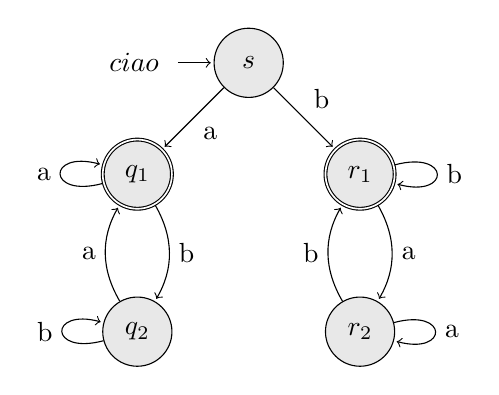
\begin{tikzpicture}[shorten >=1pt,node distance=2cm,auto]
    \tikzstyle{every state}=[fill={rgb:black,1;white,10}]

    \node[state,initial]   (s)                      {$s$};
    \node[state,accepting] (q_1) [below left of=s]  {$q_1$};
    \node[state]           (q_2) [below of=q_1]     {$q_2$};
    \node[state,accepting] (r_1) [below right of=s] {$r_1$};
    \node[state]           (r_2) [below of=r_1]     {$r_2$};

    \path[->]
    (s)   edge node {a}
    (q_1) edge node {b} (r_1)
    (q_1) edge [loop left]  node {a} (   )
    edge [bend left]  node {b} (q_2)
    (q_2) edge [loop left]  node {b} (   )
    edge [bend left]  node {a} (q_1)
    (r_1) edge [loop right] node {b} (   )
    edge [bend left]  node {a} (r_2)
    (r_2) edge [loop right] node {a} (   )
    edge [bend left]  node {b} (r_1);
    \end{tikzpicture}
\end{figure}
\end{document}